\documentclass[12pt]{article} 
\usepackage{imakeidx}
\usepackage{graphicx}
\usepackage{soul}
\usepackage{hyperref}
\usepackage{graphicx} % Necessary for images
\graphicspath{{./images/}} % Set the base path so images are more easily accessible later
\usepackage{biblatex} % To manage bibliographics information
\addbibresource{biblio_info.bib}
 
% Keep hyperlink text black and remove PDF link-border boxes.
\hypersetup{
  colorlinks=true,
  linkcolor=black,
  urlcolor=black,
  citecolor=black
}

% Make link underlines blue while keeping the text black.
\setulcolor{blue}

\title{An historical and mathematical analysis of Bitonic sorters}
\author{Pietro Marini, Michele Riolfi, Javidan Tahmazli}
\date{November 2026}

% To add a heading to the index, place its matching index command immediately after the heading and its unique \label. Use \indexsection{KEY}{LABEL}{TITLE}

% The section key describes the order among entries at the same level.
% This must be consistent with the way the sections appear in the rest of the document.

% For a section; write as the KEY a three-digit number that sets its order (001, 002, 003, ...). 

% Use \indexsubsection{SECTION-KEY}{SECTION-LABEL}{SECTION-TITLE}
% {SUBSECTION-KEY}{SUBSECTION-LABEL}{SUBSECTION-TITLE} for a subsection, and \indexsubsubsection with those same section and subsection details followed by  the subsubsection's key, label, and title. 

% Number subsection keys in the desired order within their section, and subsubsection keys within their subsection. Keep each key consistent between the parent heading and its children; make every label unique. The title arguments should match the heading text, since they are what readers see in the index.

% Use one column and the custom style file.
\makeindex[columns=1, options= -s indexstyle.ist]

% Override article's default two-column index layout.
% Because we are generating the .ind file and then inserting it, \makeindex[column=1, ...] doesn't work by itself.
% In fact, it is redundant but kept for clarity.
\makeatletter
\renewenvironment{theindex}
  {%
    \clearpage
    \section*{\indexname}%
    \@mkboth{\MakeUppercase\indexname}{\MakeUppercase\indexname}%
    \thispagestyle{plain}%
    \parindent\z@
    \parskip\z@ plus .3\p@\relax
    \let\item\@idxitem
    \normalsize
  }
  {\clearpage}
\makeatother

% Keep linked page numbers together on one line.
\let\OriginalHyperpage\hyperpage
\renewcommand*{\hyperpage}[1]{\mbox{\OriginalHyperpage{#1}}}

\setcounter{secnumdepth}{0} % Suppress heading numbers
\renewcommand{\indexname}{Index}

% Add a section entry.
% #1 is its numeric sort key; #2 its label; #3 its displayed title.
\newcommand{\indexsection}[3]{%
  \index{#1@\hyperref[#2]{\ul{#3}}}%
}

% Add a subsection beneath its parent section.
% Arguments are: section key, label, title; subsection key, label, title.
\newcommand{\indexsubsection}[6]{%
  \index{#1@\hyperref[#2]{\ul{#3}}!%
    #4@\hyperref[#5]{\ul{#6}}}%
}

% Add a subsubsection beneath its parent subsection.
% Arguments are: section key, label, title;
% subsection key, label, title; subsubsection key, label, title.
\newcommand{\indexsubsubsection}[9]{%
  \index{#1@\hyperref[#2]{\ul{#3}}!%
    #4@\hyperref[#5]{\ul{#6}}!%
    #7@\hyperref[#8]{\ul{#9}}}%
}

\begin{document}

\maketitle
\clearpage % Force new page

% Insert index.
% \printindex by itself does not work because the package only allows for the index to be at the end.
% This workaround solution makes it so MakeIndex is ran after the LaTex pass and then the generated .ind file is output in page 2.
% The two \clearpage are there just so the index has a dedicated page.
\clearpage
\IfFileExists{\jobname.ind}{\input{\jobname.ind}}{}
\clearpage

\section{History}\phantomsection\label{sec:history}
\indexsection{001}{sec:history}{History}

\subsection{Original paper}\phantomsection\label{subsec:original-paper}
\indexsubsection{001}{sec:history}{History}
                 {001}{subsec:original-paper}{Original paper}

Before discussing the original paper \cite{original_paper}, let's recall a key definition to the algorithm in question.\newline
For a sequence to be \emph{bitonic} it must satisfy one of two requirements:
\begin{itemize}
    \item it increases up to a certain element and then decreases after
    \item can be rotated in such way that it satifies the first requirement
\end{itemize}

\noindent
Before proceeding, note that, owing to its age, the paper devotes considerable attention to implementations on dedicated hardware. Here, we focus instead on the mathematical foundations, which remain applicable to modern technologies and industry standards.
The paper \cite{original_paper} begins with an introduction of the notion of sorting networks and their basic element, the comparison element.

\begin{center}
    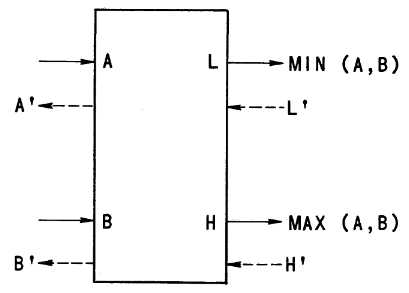
\includegraphics{comparison_element.png}
\end{center}

\noindent
Comparison elements simply gather two inputs over the inputs, A and B, and present the lowest on L and the highest on H. An additional reset input is used to place the element in the \(A=B\) state; as long as the A and B inputs agree the elements remains in this state with the outputs equal to the inputs.\newline
If the numbers are transmitted in big-endian (i.e. the MSB is the first bit) the comparison element has the following state diagram:

\begin{center}
    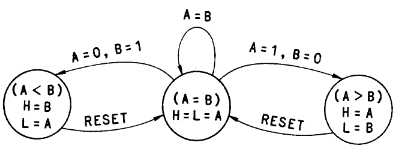
\includegraphics{comparison_element_state_diagram.png}
\end{center}

\noindent
The first kind of sorting network introduced is the odd-even merging network, as this is not the focus of this paper we'll only discuss it briefly.
Merging is the process of creating a single ordered list of numbers from two ordered lists of numbers. \newline
\newline
The key functionality of the odd-even merging network is presenting the odd-indexed elements of the two input lists to a smaller merging network, the odd merge network, presenting the even-indexed elements to a smaller merging network, the even merge network and then comparing the outputs using a row of comparison elements.\newline
Formally, let \(A = {a_1, a_2, a_3, ..., a_s}\) be an ordered list of \(s\) numbers, \(B = {b_1, b_2, b_3, ..., b_t}\) be an ordered list of \(t\) numbers.
The \(i^{th}\) output of the even merge will then compared with the \(i+1^{th}\) output of the odd merge to form the \(2i^{th}\) and \(2i+1^{th}\) elements of the final list for all applicable \(i\)'s.
The lowest output of the odd merge is left alone and will become the lowest element of the final list and, respectively, any single output not exhausted by the row of comparison elements will become the highest element of the final list.
This kind of logic can be used to construct bigger network in an iterative manner, a sketch of the formal proof is available in the Appendix A of the original paper \cite{original_paper}.\newline
In general, a "\(2^p\) by \(2^p\)" merging network built using this rule will use \((p\;*\;2^p\;)\;+\;1\) comparison elements with the longest path going through \(p+1\) elements and the shortest path through a single comparison element.\newline \newline 

\noindent
Another way of constructing merging networks is using a bitonic sorter. These kind of sorting networks require more elements than the odd-even merging networks but have the advantage of flexibility (a single network can handle input lists of various lengths) and of modularity (a large network can be split up into several identical modules recursively).
Analogously to odd-even merging networks, bitonic sorting networks can also be constructed iteratively (see Appendix B of the original paper, \cite{original_paper}).

\noindent
Let \(A = (a_1, a_2, \ldots, a_{2n})\) be a bitonic sequence of \(2n\) numbers. Define
\[
B = \bigl(\min(a_1,a_{n+1}),\, \min(a_2,a_{n+2}),\, \ldots,\, \min(a_n,a_{2n})\bigr)
\]
and
\[
C = \bigl(\max(a_1,a_{n+1}),\, \max(a_2,a_{n+2}),\, \ldots,\, \max(a_n,a_{2n})\bigr).
\]
Then \(B\) and \(C\) are bitonic sequences, and every element of \(B\) is less than or equal to every element of \(C\).
A bitonic sorting network for two numbers consists of a single comparator. By applying the iterative rule, bitonic sorting networks can be constructed for \(2^p\) numbers for any nonnegative integer \(p\). Consequently, without additional handling, bitonic sorting networks can sort only sequences whose lengths are powers of two.
A \(2^p\)-number bitonic sorter requires \(p\) levels of \(2^{p-1}\) elements each for a total of \(p*2^{p-1}\).


% Explanation not to put in the paper, just to understand better in the future:
% Take for example A = (1, 2, 3, 8, 7, 4, 3, 2). Thus, B = (min(1, 7), min(2, 4), min(3, 3), min(8, 2)) and C = (max(1, 7), max(2, 4), max(3, 3), max(8, 2)).
% Namely, B = (1, 2, 3, 2) and C = (7, 4, 3, 8).
% Of course this is just a single example but a good enough example to visualize the statement above.



 
\subsection{Related context, terminology and developments}
\phantomsection\label{subsec:related-context}
\indexsubsection{001}{sec:history}{History}
                 {002}{subsec:related-context}
                 {Related context, terminology and developments}

\subsection{Necessity and details}
\phantomsection\label{subsec:necessity}
\indexsubsection{001}{sec:history}{History}
                 {003}{subsec:necessity}{Necessity and details}

\subsection{Historical reconstruction and implementation}
\phantomsection\label{subsec:historical-reconstruction}
\indexsubsection{001}{sec:history}{History}
                 {004}{subsec:historical-reconstruction}
                 {Historical reconstruction and implementation}

\section{Validation and analysis}\phantomsection\label{sec:validation}
\indexsection{002}{sec:validation}{Validation and analysis}

\subsection{Theoretical analysis}
\phantomsection\label{subsec:theoretical-analysis}
\indexsubsection{002}{sec:validation}{Validation and analysis}
                 {001}{subsec:theoretical-analysis}{Theoretical analysis}

\subsection{Practical analysis}
\phantomsection\label{subsec:practical-analysis}
\indexsubsection{002}{sec:validation}{Validation and analysis}
                 {002}{subsec:practical-analysis}{Practical analysis}

\subsection{Complexity and performance analysis}
\phantomsection\label{subsec:complexity}
\indexsubsection{002}{sec:validation}{Validation and analysis}
                 {003}{subsec:complexity}{Complexity and performance analysis}

\subsubsection{Chosen experiments and related info}
\phantomsection\label{subsubsec:experiments}
\indexsubsubsection{002}{sec:validation}{Validation and analysis}
                    {003}{subsec:complexity}{Complexity and performance analysis}
                    {001}{subsubsec:experiments}{Chosen experiments and related info}

\section{Reality check, evolution and legacy}
\phantomsection\label{sec:reality-check}
\indexsection{003}{sec:reality-check}{Reality check, evolution and legacy}

\section{Bibliographic information}
\phantomsection\label{sec:bibliographic-info}
\indexsection{004}{sec:reality-check}{Bibliographic information}

\printbibliography[heading=none] % Print the bibliography while suppressing the heading to avoid duplicates (the integrated header in biblatex does not work properly with the custom index handling)

\end{document}
